\documentclass[slidestop]{beamer}
\usepackage{beamerthemesplit}
\usepackage{graphics}
\usepackage{pstricks}

\graphicspath{{./}}

\title{The Libre-SOC Hybrid 3D CPU}
\author{Luke Kenneth Casson Leighton}


\begin{document}

\frame{
   \begin{center}
    \huge{The Libre-SOC Hybrid 3D CPU}\\
    \vspace{32pt}
    \Large{Draft SVP64 in-place Matrix Multiply}\\
    \Large{and FFT / DCT for the Power ISA}\\
    \vspace{24pt}
    \Large{OpenPOWER Summit 2021}\\
    \vspace{16pt}
    \large{Sponsored by NLnet's PET Programme}\\
    \vspace{6pt}
    \large{28th Oct 2021}
  \end{center}
}


\frame{\frametitle{}

\vspace{15pt}

 \begin{itemize}
   \item \vspace{15pt}
   \item \vspace{15pt}
   \item \vspace{15pt}
  \end{itemize}
}

\frame{\frametitle{Overview of Libre-SOC goals}

\vspace{15pt}

 \begin{itemize}
   \item To create power-efficient mass-volume products\vspace{15pt}
   \item To leverage the OpenPOWER ecosystem to do so\vspace{15pt}
   \item To be entirely transparent for Security reasons\vspace{15pt}
   \item To empower businesses to bring Secure transparent\\
         mass-volume products to market\vspace{15pt}
  \end{itemize}
}

\frame{\frametitle{Overview of SVP64 goals}

\vspace{15pt}

 \begin{itemize}
   \item High performance and high performance/watt\vspace{15pt}
   \item Reduced code density (reduced I-Cache usage)\\
         https://arxiv.org/abs/2002.10143 - 3.5x power reduction\vspace{8pt}
   \item Remain accessible for assembler writers and compilers alike\vspace{15pt}
   \item Introduce true Vectorisation to the Power ISA\\
         (VSX is Packed SIMD)\vspace{8pt}
   \item Be adopted via the external OPF ISA WG RFC process\\
         (not: be a non-official custom extension. proprietary\\
         custom extensions conflict with mass-volume adoption)\vspace{15pt}
  \end{itemize}
}



%%\frame{\frametitle{nmigen PowerISA Decoder}

%%\begin{center}
%%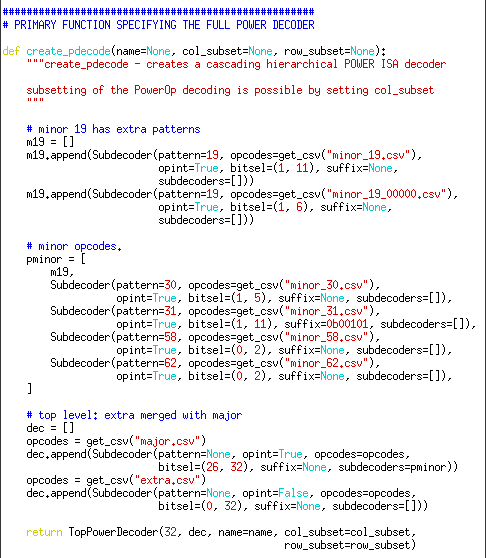
\includegraphics[width=0.55\textwidth]{2020-09-09_21-04.png}
%%\end{center}

%%}

\begin{frame}[fragile]
\frametitle{Reminder of Simple-V}

\begin{semiverbatim}
Greatly simplified (like x86 "REP" instruction):

  for (i = 0; i < VL; i++)
       ireg[RT+i] <= ireg[RA+i] + ireg[RB+i];

function op\_add(rd, rs1, rs2, predr) # add not VADD!
  int i, id=0, irs1=0, irs2=0;
  for (i = 0; i < VL; i++)
    if (ireg[predr] & 1<<i) # predication uses intregs
       ireg[rd+id] <= ireg[rs1+irs1] + ireg[rs2+irs2];
    if (reg\_is\_vectorised[rd] )  \{ id += 1; \}
    if (reg\_is\_vectorised[rs1])  \{ irs1 += 1; \}
    if (reg\_is\_vectorised[rs2])  \{ irs2 += 1; \}
\end{semiverbatim}

\end{frame}



\frame{\frametitle{Summary}

 \begin{itemize}
   \item Goal is to create a mass-volume low-power embedded SoC suitable
         for use in netbooks, chromebooks, tablets, smartphones, IoT SBCs.
   \item No DRM. 'Trustable' (by the users, not by Media Moguls) design
         ethos as a \textit{business} objective: requires full transparency
         as well as Formal Correctness Proofs
   \item Collaboration with OpenPOWER Foundation and Members absolutely
         essential. No short-cuts.  Standards to be developed and ratified
         so that everyone benefits.
   \item Working on the back of huge stability of POWER ecosystem
   \item Combination of which is that Board Support Package is 100\%
         upstream, app and product development by customer is hugely
         simplified and much more attractive
         
  \end{itemize}
}


\frame{
  \begin{center}
    {\Huge The end\vspace{15pt}\\
		   Thank you\vspace{15pt}\\
		   Questions?\vspace{15pt}
	}
  \end{center}
  
  \begin{itemize}
	\item Discussion: Libre-SOC-dev mailing list
	\item Freenode IRC \#libre-soc
	\item http://libre-soc.org/
	\item http://nlnet.nl/PET
  \end{itemize}
}


\end{document}
